The Beneš network is an extension of the Banyan network.
It solves the problem that a Banyan network is not able to produce all possible permutations by mirroring the Banyan network and connecting the two.
An example for a Beneš network with 8 inputs is given in Figure \ref{fig:benes}.

The two halves of the network are different in the routing procedure employed.
For the output half, the destination of a data packet defines the exact setting of every switch on its path, because there always is only one possible choice.
The input half is responsible for conflict avoidance, which has a significantly higher complexity due to the fact that it depends on all inputs of one column of the network.

For implementation, the recursive structure given in Figure \ref{fig:benes_recursion} was used.
A network with $2^n$ inputs is defined as $benes(n, n)$, where the first parameter gives the size of the specific network defined, and the second is used during recursion to remember the size of the whole network.

For this structure, the routing decision of the output switches is based on just bit $k - 1$, where a $0$ requires the packet to go up and $1$ to go down.

\begin{figure}[!ht]
	\centering
	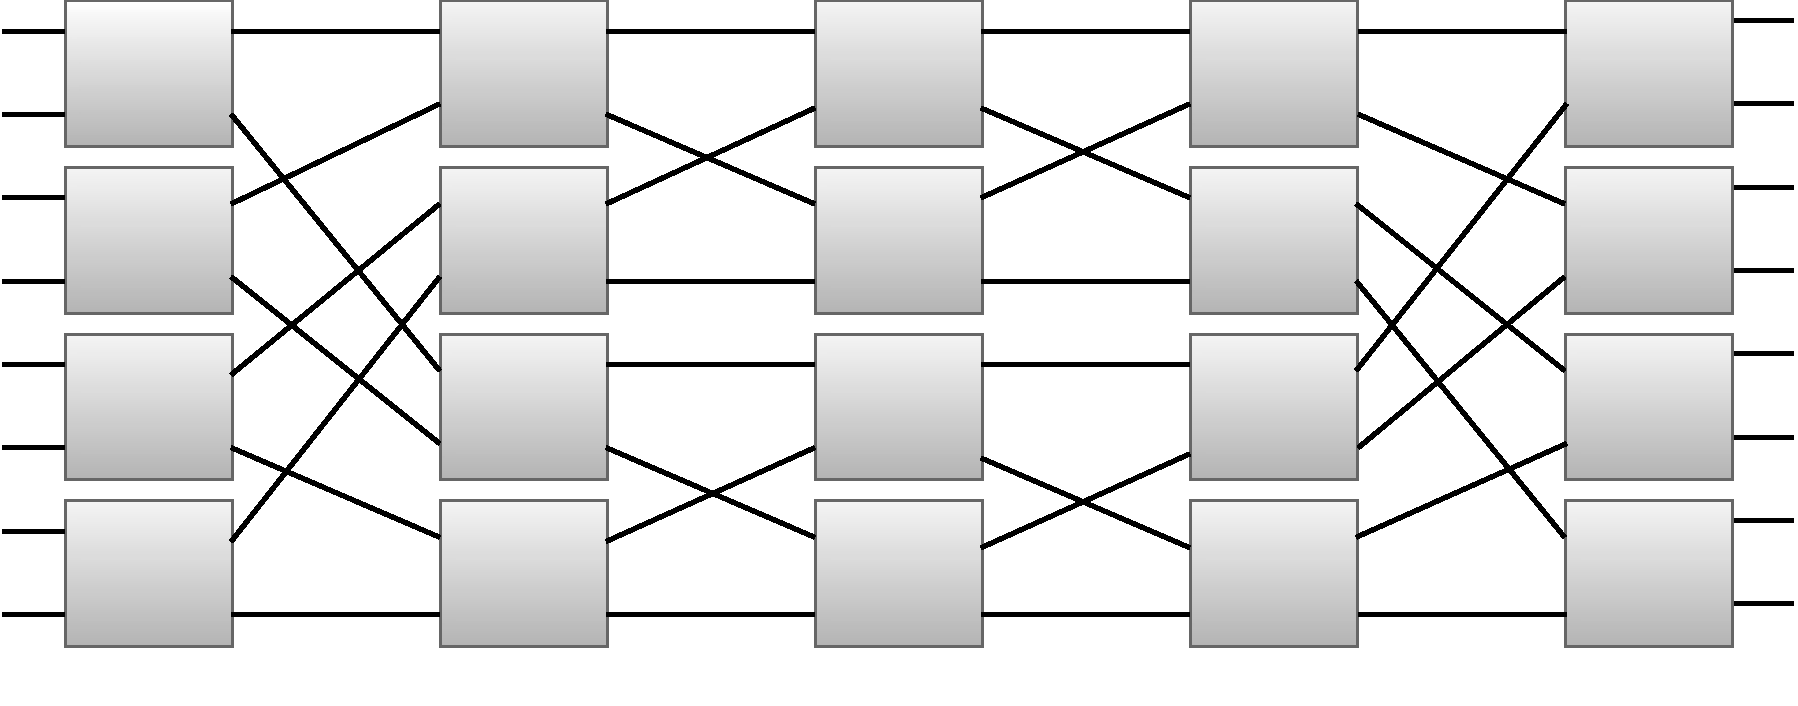
\includegraphics[width=0.7\linewidth]{benes_network.pdf}
	\caption{The basic structure of a Beneš network}
	\label{fig:benes}
\end{figure}


\begin{figure}[!ht]
	\centering
	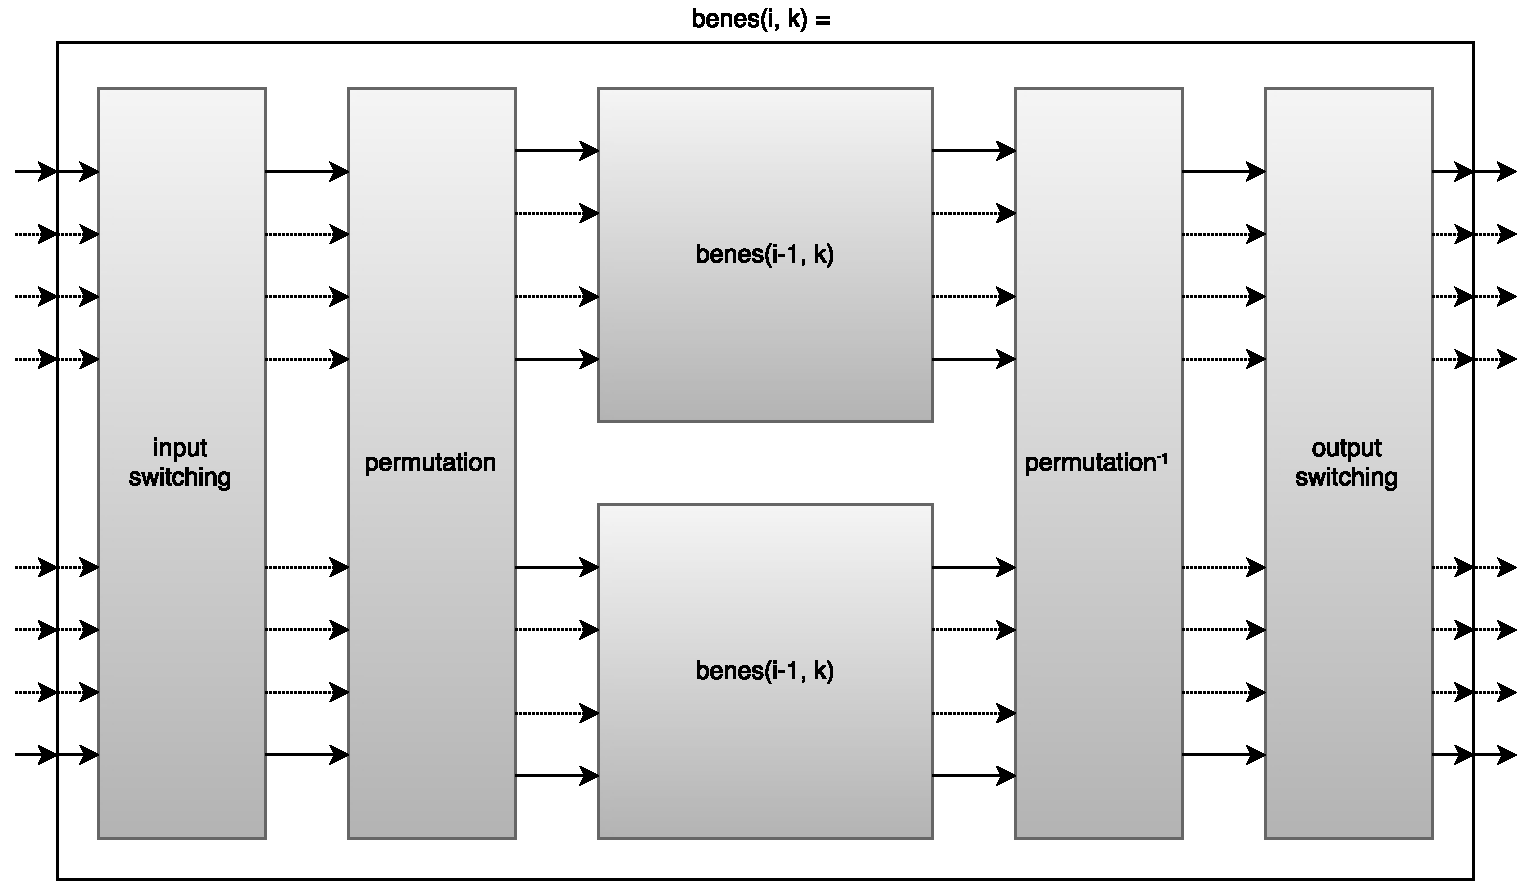
\includegraphics[width=0.7\linewidth]{benes_recursion.pdf}
	\caption{Recursive definition of a Beneš network}
	\label{fig:benes_recursion}
\end{figure}

\begin{figure}[!ht]
	\centering
	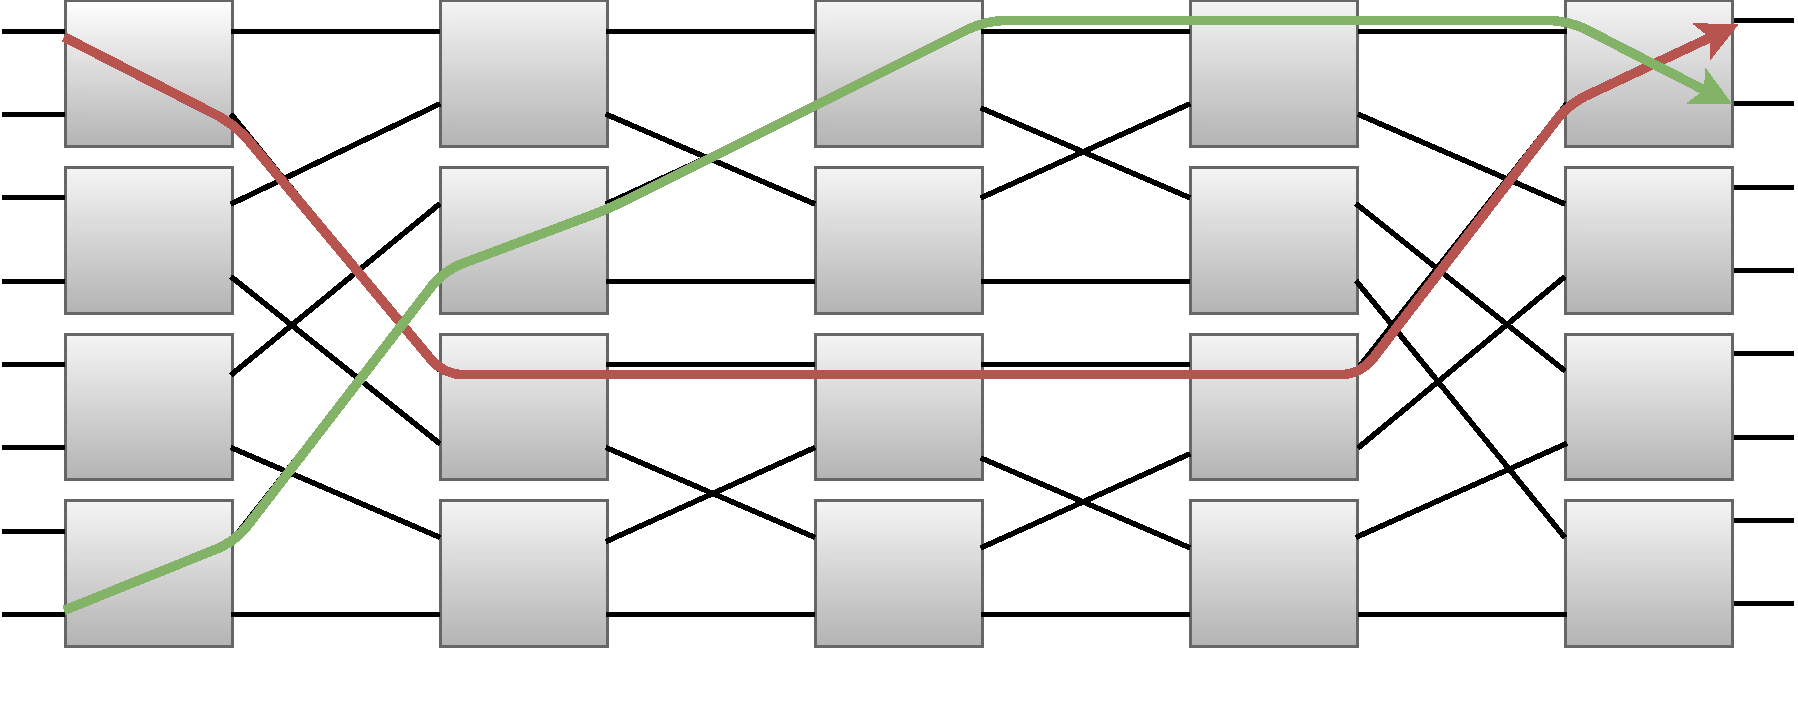
\includegraphics[width=0.7\linewidth]{benes_companions.pdf}
	\caption{Paths of two outermost-layer companions}
	\label{fig:benes_companions}
\end{figure}

\begin{figure}[!ht]
	\centering
	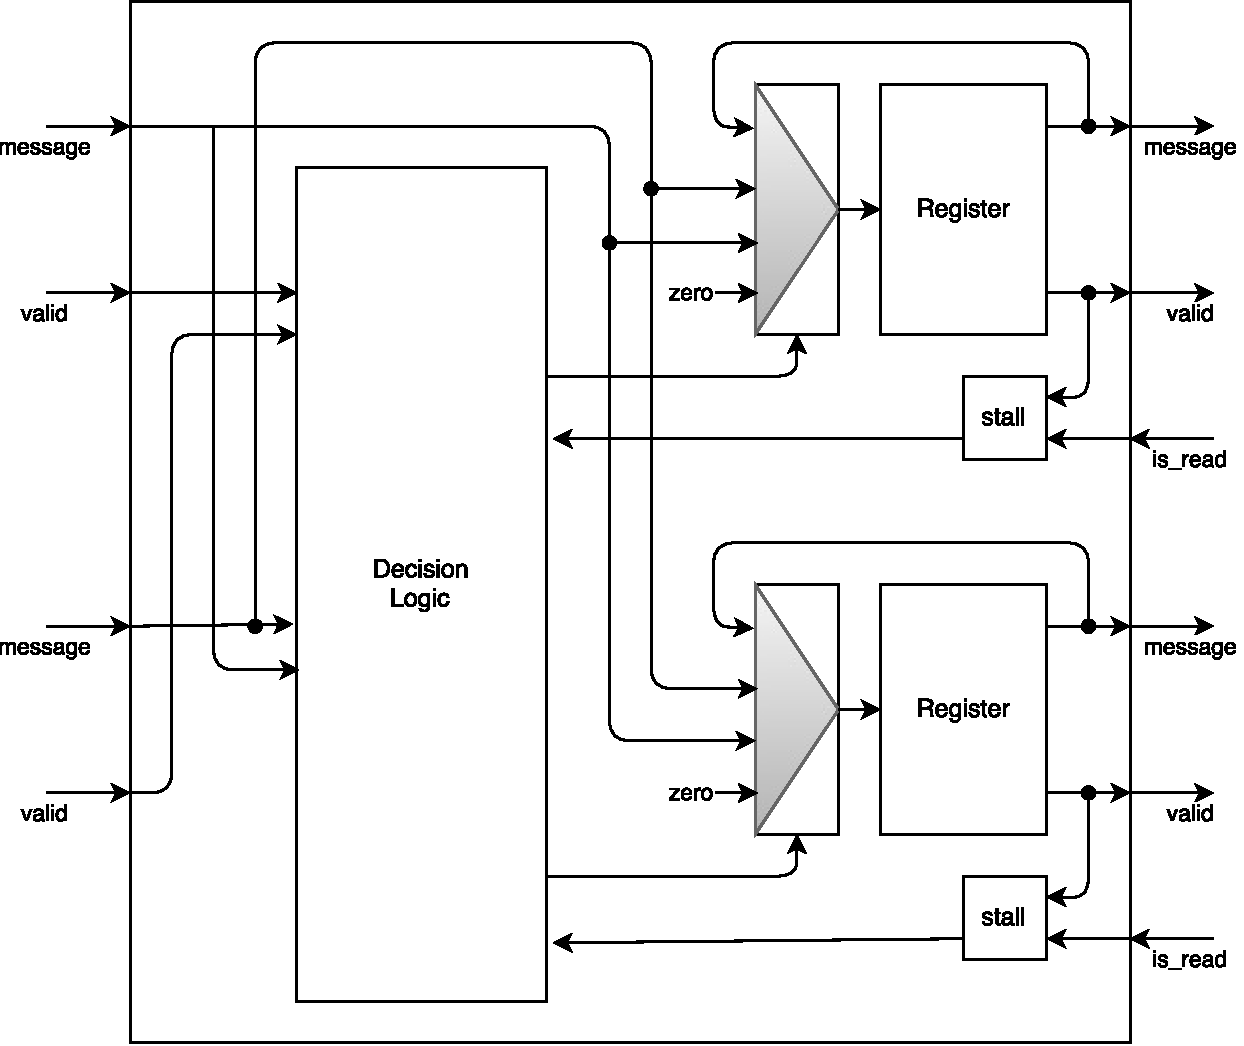
\includegraphics[width=0.7\linewidth]{banyan_stall_switch.pdf}
	\caption{Structur of stalling banyan network switches}
	\label{fig:banyan_stall_switch}
\end{figure}

\begin{figure}[!ht]
	\centering
	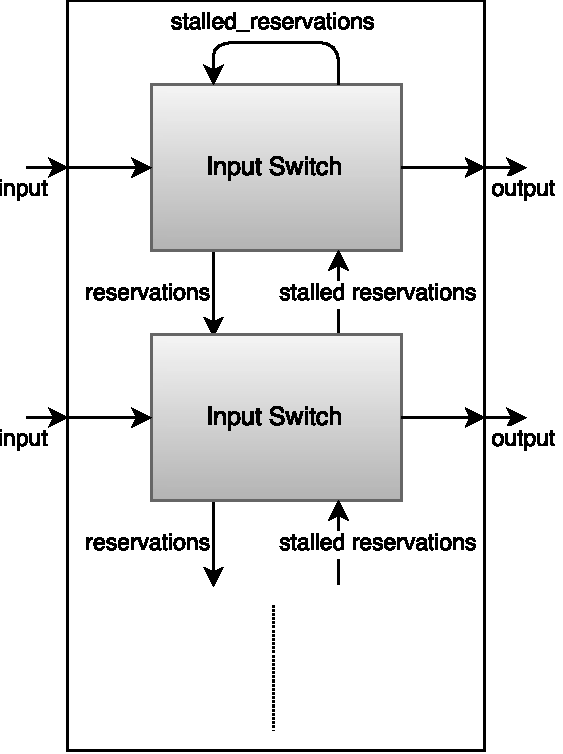
\includegraphics[width=0.3\linewidth]{benes_input_column.pdf}
	\caption{Structur of Beneš network input switch column}
	\label{fig:benes_switchcolumn_in}
\end{figure}

\begin{figure}[!ht]
	\centering
	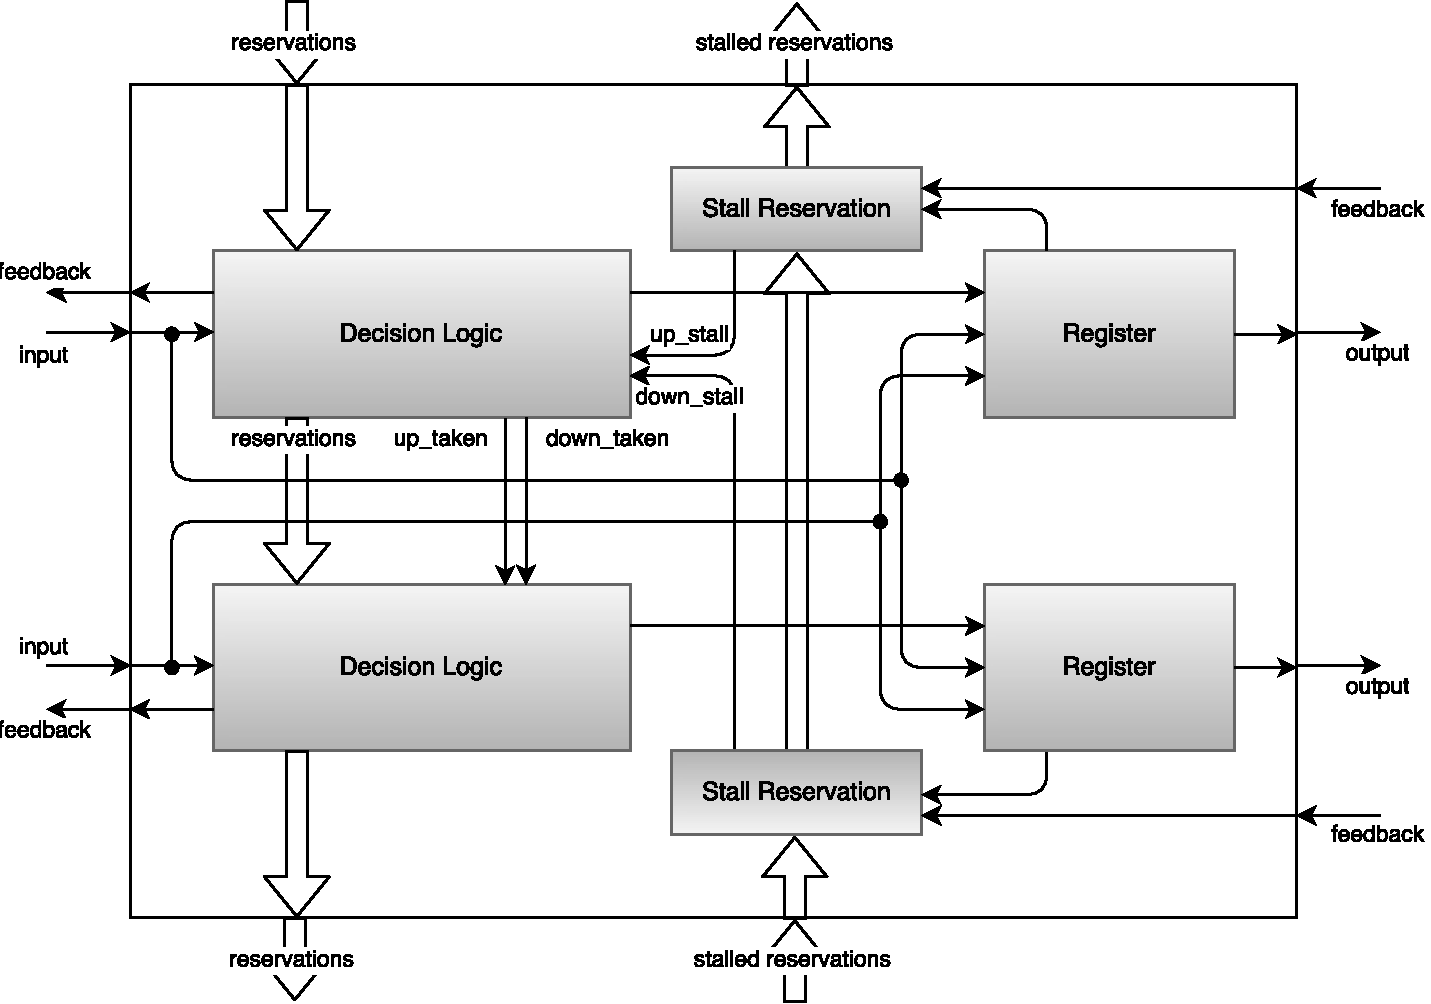
\includegraphics[width=0.8\linewidth]{benes_input_switch.pdf}
	\caption{Functional overview of Beneš input switch}
	\label{fig:benes_switch_in}
\end{figure}

\todo{move this} A lookup table for the first stage of a $32\times32$ benes network would require around $2.92\times10^{48}$ bytes.

\subsubsection{Message Ordering}

		For each packet from source $s$ and destination $d$ and for the program order of move instructions $m_n(s_n, d_n) \prec m_{n+1}(s_{n+1}, d_{n+1})$, and delivery order of network $m_n \lhd m_k$, the following constraint has to hold:
	\begin{align*}
		& $(m_n(s_n, d_n) \prec m_k(s_k, d_k)) \wedge (s_n = s_k \wedge d_n = d_k) \\
		& \Rightarrow (m_n(s_n, d_n) \lhd m_k(s_k, d_k))$
	\end{align*}

	This is necessary since the input buffers cannot distinguish between different packets that have equal sources and destinations.
	
	With the recursive structure of the Beneš network and possible stalling at each input step, this constraint can not be guaranteed and is a case for which the network might work incorrectly.
	This does not apply to the Banyan part of the network, since relevant message pairs take the same path and do not overtake each other.
	
